
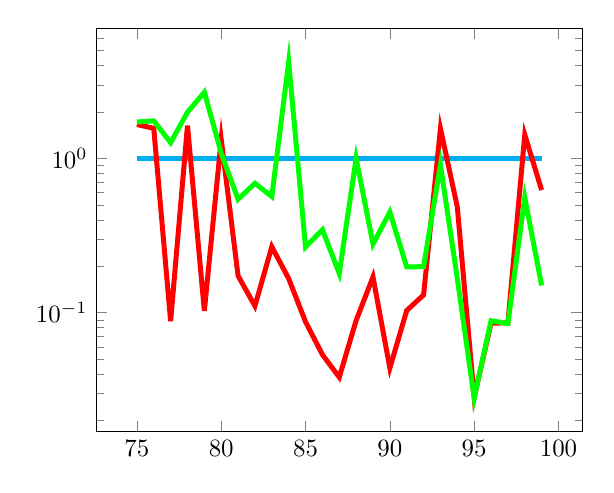
\begin{tikzpicture}[scale=0.9]
\begin{semilogyaxis}
\addplot[color=cyan,line width=2pt] coordinates {(75,1.0)(76,1.0)(77,1.0)(78,1.0)(79,1.0)(80,1.0)(81,1.0)(82,1.0)(83,1.0)(84,1.0)(85,1.0)(86,1.0)(87,1.0)(88,1.0)(89,1.0)(90,1.0)(91,1.0)(92,1.0)(93,1.0)(94,1.0)(95,1.0)(96,1.0)(97,1.0)(98,1.0)(99,1.0)};
\addplot[color=red,line width=2pt] coordinates {(75,1.6582987559201914)(76,1.5660223283521923)(77,0.08808967408826456)(78,1.6331095898659516)(79,0.10280919580216386)(80,1.3271086168223585)(81,0.1734513541991085)(82,0.11057700080435325)(83,0.2676917188956431)(84,0.16632033241520575)(85,0.08735215392146045)(86,0.05353434104784764)(87,0.03820850675128932)(88,0.08903586476201616)(89,0.17048893010850633)(90,0.043793598425095996)(91,0.10333631851232306)(92,0.13038824962112142)(93,1.560952884817941)(94,0.48467030396725924)(95,0.028371291106201176)(96,0.08551974948435104)(97,0.08601019474258076)(98,1.4240582450080483)(99,0.6235484482350153)};
\addplot[color=green,line width=2pt] coordinates {(75,1.7224489411121418)(76,1.7503672868364621)(77,1.264756770127282)(78,1.9928960721323319)(79,2.6836026820304326)(80,1.0827442757576535)(81,0.5430755622094539)(82,0.6897299634948598)(83,0.5660839557141931)(84,4.227042377826975)(85,0.2667241094489211)(86,0.34524456841887224)(87,0.17964984222785493)(88,1.0002541078875307)(89,0.27883338241764094)(90,0.4495289415986157)(91,0.19811056017458284)(92,0.1988581184475629)(93,0.9080470010082672)(94,0.16622326121271702)(95,0.028001299246058167)(96,0.08875122664709832)(97,0.0850669775745634)(98,0.5585456858660877)(99,0.15002748163942192)};

\end{semilogyaxis}
\end{tikzpicture}
